\documentclass{article}

% anonymous submission to extended abstract track
\usepackage[review,eabstract]{log_2026}

\usepackage{booktabs}       % professional-quality tables
\usepackage{amsfonts}       % blackboard math symbols
\usepackage{nicefrac}       % compact symbols for 1/2, etc.
\usepackage{graphicx}       % required for figures
\usepackage{float}          % required for exact [H] float placement

\title{Grokking Breadth-First Search: Generalizing from 16 to 1600 Nodes with Pointer Graph Networks}

\author[M. Milenkovi\'{c}]{%
  Marko Milenkovi\'{c} \\
  Faculty of Technical Sciences, University of Novi Sad\\
  \email{mmarkomile@gmail.com}
}

\begin{document}

\maketitle

\begin{abstract}
Neural Algorithmic Reasoning (NAR) models are increasingly being pushed to their limits to test out-of-distribution (OOD) generalization, often failing when evaluated on graphs significantly larger than those seen during training. In this extended abstract, we propose a heavily regularized Pointer Graph Network (PGN) training pipeline for the Breadth-First Search (BFS) task within the SALSA-CLRS benchmark. By combining Autoregressive Teacher Forcing (AR+TF), hidden state noise injection, and aggressive weight decay within a low-variance, high-batch-size grokking regime, we achieve extreme OOD generalization. Training exclusively on Erd\H{o}s-R\'{e}nyi (ER) graphs of $N \le 16$ nodes, our best run maintains $100\%$ exact graph match accuracy on structurally distinct Delaunay triangulations of 1600 nodes when evaluated at full numerical precision ($95.5\% \pm 9.0\%$ across grokked seeds). Crucially, this marks a categorical improvement over the standard SALSA-CLRS PGN baseline, which collapses to near-zero ($\le 0.2\%$) graph accuracy at these scales. This 100x scale increase in evaluation size demonstrates highly robust algorithmic alignment. Our results provide evidence that, at least for BFS, standard GNNs already possess significant latent capacity for extreme algorithmic generalization, challenging the assumption that highly specialized architectural biases are necessary for robust extrapolation on this task.
\end{abstract}

\section{Introduction}

Standard Graph Neural Networks (GNNs) \cite{velickovic2020pointer} are highly capable of algorithmic interpolation but frequently fail when forced to extrapolate execution traces to massive out-of-distribution (OOD) graphs \cite{velickovic2022clrs}. The SALSA-CLRS benchmark \cite{minder2023salsa} formalizes this frontier, pushing evaluation limits up to 100x the training distribution to expose the fragility of learned heuristics. To overcome these severe OOD bottlenecks, recent state-of-the-art research has increasingly focused on developing novel, discrete, or highly specialized neural architectures. For example, recent works introduce custom structural biases or algorithm-specific network layers, such as FloydNet \cite{floydnet} and other recent specialized topologies \cite{rodionov2025discrete}, to force strict algorithmic alignment. 

We present empirical evidence suggesting that such drastic architectural overhauls may not always be strictly necessary. We demonstrate that ordinary GNN baselines---specifically the standard Pointer Graph Network (PGN) \cite{velickovic2020pointer}---already possess the representational capacity required for extreme OOD scaling. The true bottleneck is often a mechanical breakdown in the optimization trajectory. We observe that successful OOD generalization in these tasks empirically mirrors a ``grokking'' phase transition \cite{power2022grokking}, relying on a fragile equilibrium between data-driven memorization and regularization-driven compression. By systematically optimizing the training pipeline of the SALSA-CLRS baseline without fundamentally altering the core architecture, we achieve 100x OOD scaling. Mechanistic ablations justifying these optimization requirements are provided in Appendix \ref{sec:ablations}.

\section{Methodology}

\subsection{Architectural Enhancements}
To prevent hidden state decay over exponentially longer sequence rollouts, we integrate a Gated Recurrent Unit (GRU) to act as a persistent algorithmic memory bank. Furthermore, we inject latent Gaussian noise ($\sigma = 0.015$) directly into the hidden state embeddings during training. We hypothesize that this noise acts as a structural regularizer, forcing the network to learn a wide, self-correcting memory basin. This robustness is critical for OOD generalization, as it prevents microscopic prediction errors from compounding and derailing the network during extended autonomous inference loops on graphs of up to 1600 nodes.

\subsection{Optimization and Scaffolding}
To combat exposure bias, instead of pure Teacher Forcing, we use an Autoregressive and Teacher Forcing (AR+TF) blend, applying a $0.4$ hint dropout rate to force autonomous execution recovery. 

To drive the sudden leap in algorithmic alignment, we employ a strict optimization regimen. We utilize the AdamW optimizer with an aggressive weight decay ($\lambda=0.09$) to force the network to compress its initial memorization circuit into sparse, generalizable logic. Because discrete algorithmic routing is highly brittle to stochastic updates, we physically suppress gradient variance by training with a massive static batch size ($\mathcal{B}=2048$).

\section{Main Results}

Models were trained exclusively on Erd\H{o}s-R\'{e}nyi (ER) graphs restricted to $N \le 16$ nodes. Evaluations were conducted tracking both strict full-sequence \texttt{graph\_accuracy} and local \texttt{node\_accuracy} across topologies.

As detailed in Table~\ref{results-table}, our optimized pipeline yields a categorical leap in OOD performance compared to the SALSA-CLRS baseline. Where the baseline PGN completely collapses on strict graph accuracy at $N=800$, our model maintains perfect $1.000$ accuracy on ER and Delaunay graphs. At the extreme 100x scale ($N=1600$), our best run retains $100.0\%$ accuracy on structurally distinct Delaunay graphs (compared to the baseline's $0.0\%$), and $95.5\% \pm 9.0\%$ across the five runs that grokked (Appendix~\ref{sec:perseed}). Watts-Strogatz (WS) remains the hardest family: $98.0\%$ at $N=1600$ for our best run, with large variance across seeds.

An earlier version of this abstract reported substantially lower numbers ($80.0\%$ on Delaunay-1600 and $0.0\%$ on WS-1600). Those values were an artefact of evaluating at reduced arithmetic precision (fp16 autocast with reduced-precision matmuls, neither of which was stated); the model weights are unchanged. Table~\ref{results-table} reports the same frozen model evaluated at full fp32 over 200 graphs per bin. Accuracy is monotone in evaluation precision in every bin, and \texttt{node\_accuracy} at full precision is $100.0\%$ across all topologies at the 100x scale (per-seed results and the precision analysis are in Appendix~\ref{sec:perseed}; a long-rollout path-graph evaluation is in Appendix~\ref{sec:pathgraphs}). While the baseline's \texttt{node\_accuracy} severely degrades at $N=1600$ (falling to $40.8\%$ on Delaunay), our pipeline's underlying algorithmic representation remains exact.

\begin{table}[H]
  \caption{Comparison of Strict Graph Accuracy and Node Accuracy (\%) between the SALSA-CLRS Baseline PGN (with hints) and Our PGN Pipeline. Models were trained on ER graphs of $N \le 16$. \textbf{Ours}: best checkpoint, evaluated at full fp32 precision (fp32 matmuls), 200 graphs per bin; the spread across grokked seeds is given in Appendix~\ref{sec:perseed}. \textbf{Base}: as reported by SALSA-CLRS.}
  \label{results-table}
  \centering
  \resizebox{\textwidth}{!}{%
  \begin{tabular}{lcccccccccccc}
    \toprule
    & \multicolumn{4}{c}{\textbf{Erd\H{o}s-R\'{e}nyi (ER)}} & \multicolumn{4}{c}{\textbf{Delaunay}} & \multicolumn{4}{c}{\textbf{Watts-Strogatz (WS)}} \\
    \cmidrule(r){2-5} \cmidrule(r){6-9} \cmidrule(r){10-13}
    & \multicolumn{2}{c}{Graph Acc.} & \multicolumn{2}{c}{Node Acc.} & \multicolumn{2}{c}{Graph Acc.} & \multicolumn{2}{c}{Node Acc.} & \multicolumn{2}{c}{Graph Acc.} & \multicolumn{2}{c}{Node Acc.} \\
    \cmidrule(r){2-3} \cmidrule(r){4-5} \cmidrule(r){6-7} \cmidrule(r){8-9} \cmidrule(r){10-11} \cmidrule(r){12-13}
    \textbf{Nodes ($N$)} & Base & \textbf{Ours} & Base & \textbf{Ours} & Base & \textbf{Ours} & Base & \textbf{Ours} & Base & \textbf{Ours} & Base & \textbf{Ours} \\
    \midrule
    $N=16$ & 100.0 & \textbf{100.0} & 100.0 & \textbf{100.0} & 100.0 & \textbf{100.0} & 100.0 & \textbf{100.0} & 100.0 & \textbf{100.0} & 100.0 & \textbf{100.0} \\
    $N=80$      & 88.1  & \textbf{100.0} & 99.8  & \textbf{100.0} & 26.2  & \textbf{100.0} & 97.5  & \textbf{100.0} & 14.2  & \textbf{100.0} & 96.1  & \textbf{100.0} \\
    $N=800$    & 0.2   & \textbf{100.0} & 98.7  & \textbf{100.0} & 0.1   & \textbf{100.0} & 53.2  & \textbf{100.0} & 0.0   & \textbf{99.5}  & 76.4  & \textbf{100.0} \\
    $N=1600$  & 0.0   & \textbf{99.5}  & 98.5  & \textbf{100.0} & 0.0   & \textbf{100.0} & 40.8  & \textbf{100.0} & 0.0   & \textbf{98.0}  & 80.6  & \textbf{100.0} \\
    \bottomrule
  \end{tabular}%
  }
\end{table}

To evaluate the stability of our heavily regularized pipeline, we conducted a multiseed evaluation across 10 independent training runs. Because the grokking phenomenon relies on escaping a local minimum to trigger a discrete phase transition, it is inherently sensitive to initialization. In our evaluation, 5 out of the 10 runs successfully grokked. Grokked runs were identified from the validation curves in Figure~\ref{fig:multiseed_combined}; this involves no judgement call, as the population is cleanly bimodal: maximum training weight norm reaches $196$--$268$ for grokked runs versus $56$--$160$ for the rest, so any threshold in between yields the same $5/10$ split without reference to test data. This phase transition is visually confirmed in Figure~\ref{fig:multiseed_combined} (top), where the successful runs exhibit a sudden, sharp increase in the network's weight norm, escaping the penalty phase to build high-capacity representations. Concurrently, as demonstrated in Figure~\ref{fig:multiseed_combined} (bottom), these 5 successful runs align precisely with a spike to near-perfect validation node accuracy on the highly demanding Watts-Strogatz (WS-800) topology. This confirms that when the optimization trajectory successfully navigates the phase transition, the resulting algorithmic alignment is both robust and reproducible.

\subsection{Grokking Dynamics and Margin Maximization}

While standard grokking often exhibits a regularization-driven \textit{drop} in weight norm \cite{power2022grokking}, our pipeline produces an uncharacteristic spike. We hypothesize this is driven by margin maximization within the discrete routing context. Pointer Graph Networks must approximate a hard argmax using a continuous softmax. During the memorization phase, the $L_2$ penalty restricts capacity. However, upon discovering a perfectly generalizing algorithmic circuit, the features become linearly separable. The cross-entropy gradient---pushing to maximize the margin for the correct pointer---overcomes the quadratic weight penalty. The model rapidly scales its weights to confidently simulate discrete logic, driving the weight norm spike.

\begin{figure}[htbp]
  \centering
  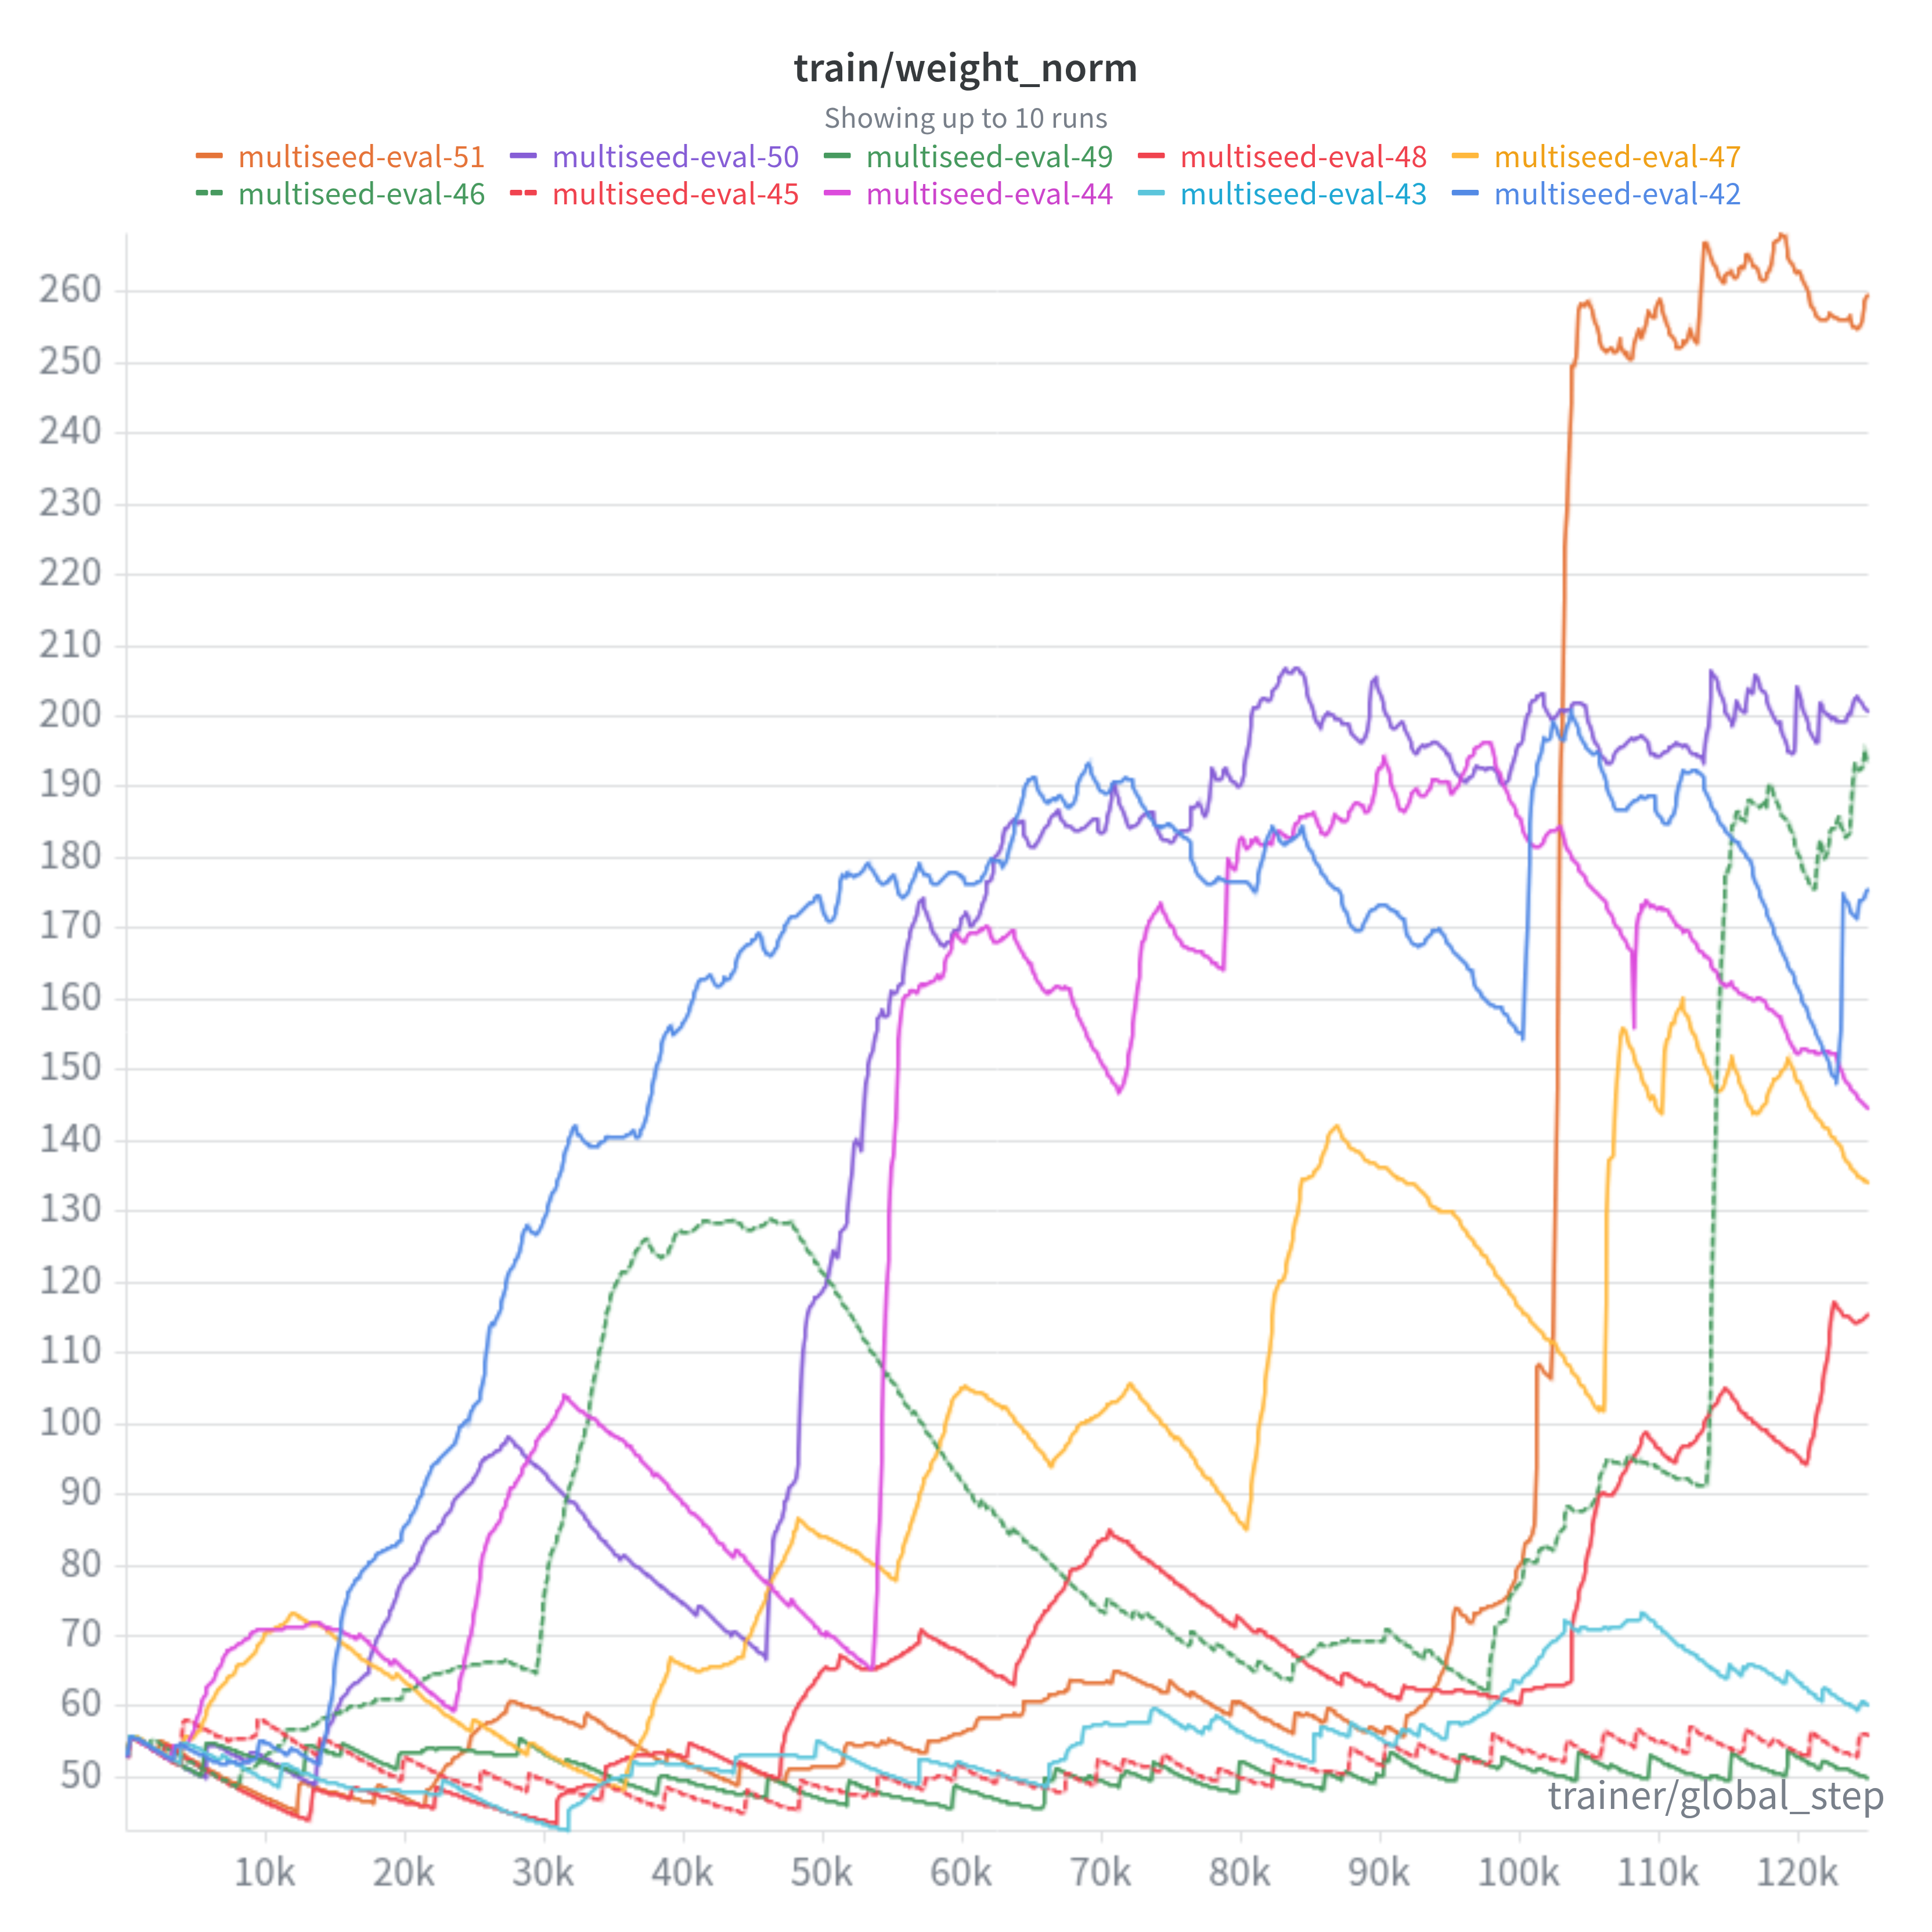
\includegraphics[width=0.75\textwidth]{multiseed_weight_norm.png}
  
  \vspace{0.3cm}
  
  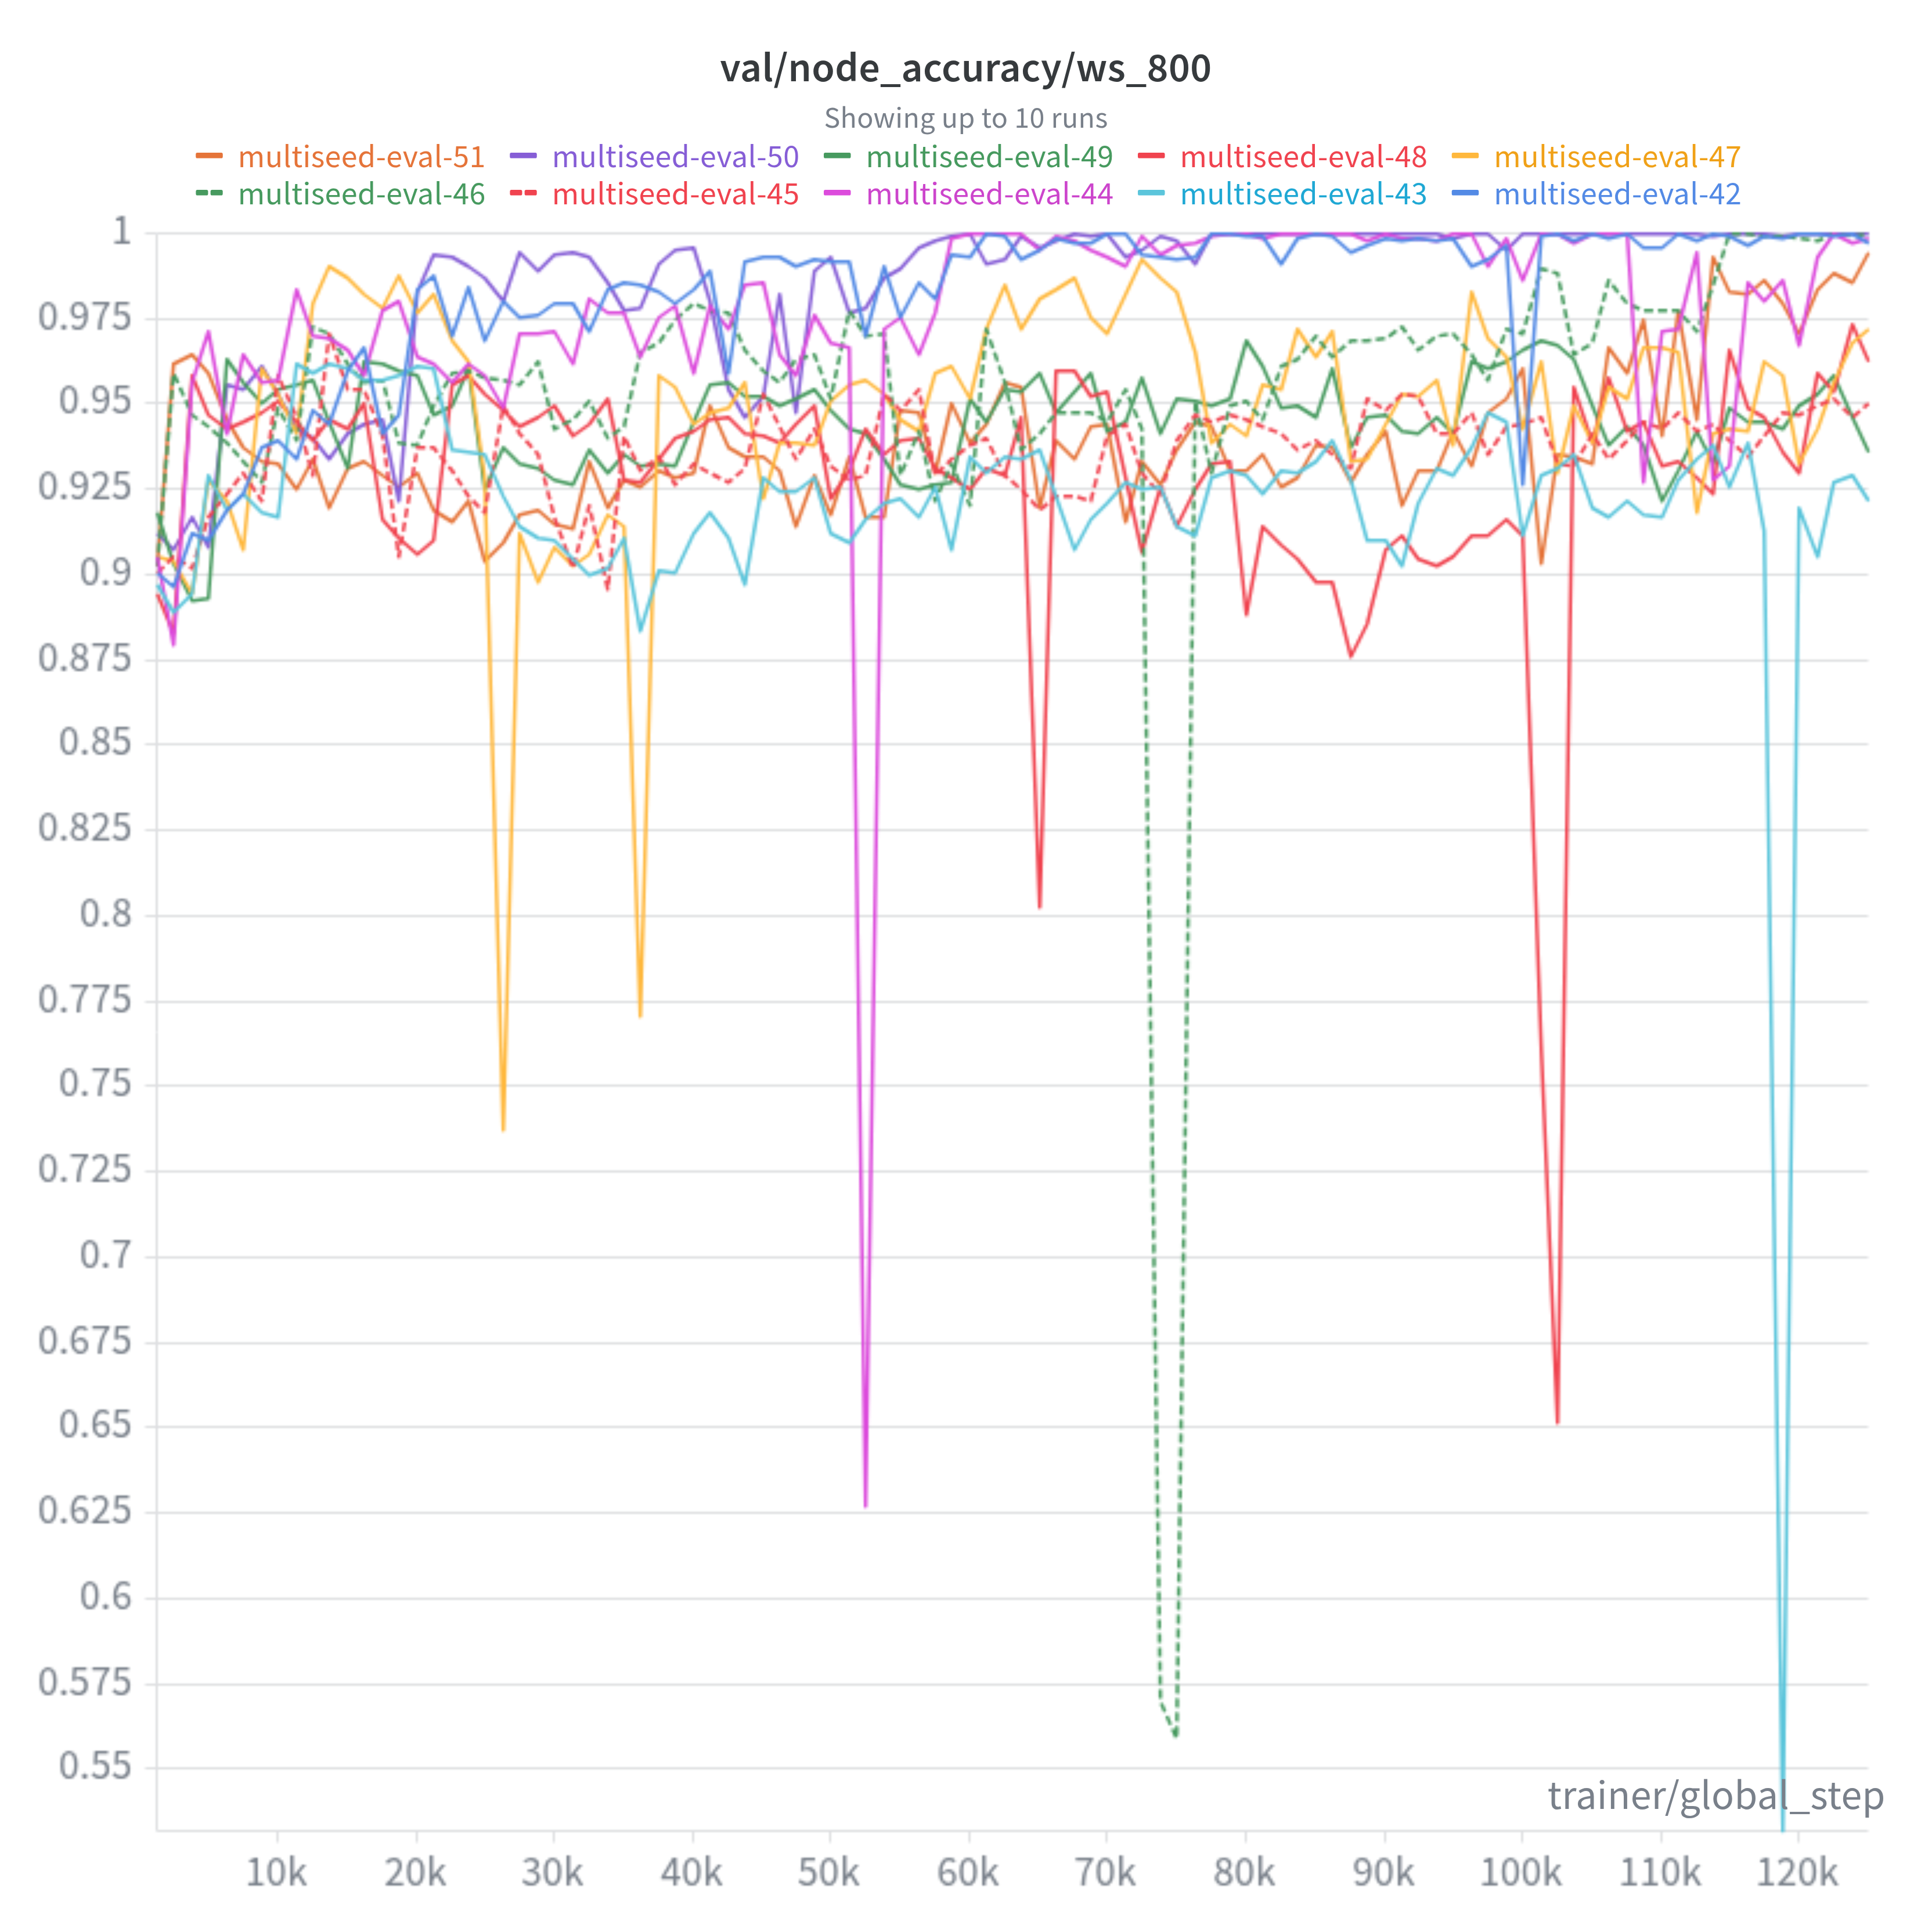
\includegraphics[width=0.75\textwidth]{multiseed_ws_node.png}
  \caption{Multiseed evaluation across 10 independent training runs. \textbf{Top:} Training weight norm ($||w||$) progression, demonstrating 5 of the 10 runs successfully transitioning to a high-capacity state. \textbf{Bottom:} Validation Node Accuracy on the WS-800 topology for the same 10 seeds, showing near-perfect local routing stability precisely aligning with the 5 runs that grokked.}
  \label{fig:multiseed_combined}
\end{figure}

\section{Conclusion}
Our empirical results demonstrate that ordinary GNNs already possess the representational capacity necessary for extreme algorithmic generalization. The primary bottleneck lies in the optimization trajectory. Successful algorithmic learning benefits greatly from deviating from standard deep learning heuristics: our models relied on an ultra-low-variance optimization environment, hidden state noise, and dense execution trace scaffolding to successfully construct and compress strict algorithmic logic. For BFS, mechanically aligning the optimization in this way was sufficient to elicit exact algorithmic behaviour from a standard graph architecture; whether the recipe transfers to harder algorithms remains open.

\clearpage
\begin{thebibliography}{9}

\bibitem{velickovic2022clrs}
Veli\v{c}kovi\'{c}, P., et al. (2022). 
\textit{The CLRS Algorithmic Reasoning Benchmark}. 
In Proceedings of the 39th International Conference on Machine Learning (ICML).

\bibitem{minder2023salsa}
Minder, J., Gr\"{o}tschla, F., Mathys, J., \& Wattenhofer, R. (2023). 
\textit{SALSA-CLRS: A Sparse and Scalable Benchmark for Algorithmic Reasoning}. 
In 2nd Learning on Graphs Conference (LoG).

\bibitem{velickovic2020pointer}
Veli\v{c}kovi\'{c}, P., Buesing, L., Overlan, M., Pascanu, R., Vinyals, O., \& Blundell, C. (2020). 
\textit{Pointer Graph Networks}. 
Advances in Neural Information Processing Systems (NeurIPS).

\bibitem{floydnet}
Yu, J., Zeng, M., \& Ye, Q. (2026). 
\textit{FloydNet: A Learning Paradigm for Global Relational Reasoning}. 
arXiv preprint arXiv:2601.19094.

\bibitem{power2022grokking}
Power, A., Burda, Y., Edwards, H., Babuschkin, I., \& Misra, V. (2022). 
\textit{Grokking: Generalization Beyond Overfitting on Small Algorithmic Datasets}. 
arXiv preprint arXiv:2201.02177.

\bibitem{rodionov2025discrete}
Rodionov, G., \& Prokhorenkova, L. (2025). 
\textit{Discrete Neural Algorithmic Reasoning}. 
In International Conference on Machine Learning (ICML) (pp. 51851-51865). PMLR.

\end{thebibliography}

\clearpage
\appendix

\section{Mechanistic Ablations}
\label{sec:ablations}

We conducted several ablations against our optimized baseline to isolate the physical drivers of algorithmic phase transitions.

\subsection{The Role of Optimization Noise ($\mathcal{B}=8$ vs $\mathcal{B}=2048$)}

As illustrated in Figure \ref{fig:weight_norm}, high stochastic optimization noise actively undermines algorithmic alignment. In our $\mathcal{B}=8$ ablation (\texttt{ablation-scheduler-smallbs}), the model's weight norm prematurely plateaus ($||w|| \approx 75$), suggesting a physical failure to construct the high-norm representations ($||w|| \approx 200$ in our \texttt{best-model} baseline) that characterize successful alignment in this regime. We hypothesize that this lower-capacity state was insufficient to withstand the aggressive $0.09$ weight decay, preventing the model from transitioning from local heuristics to global logic.

\begin{figure}[htbp]
  \centering
  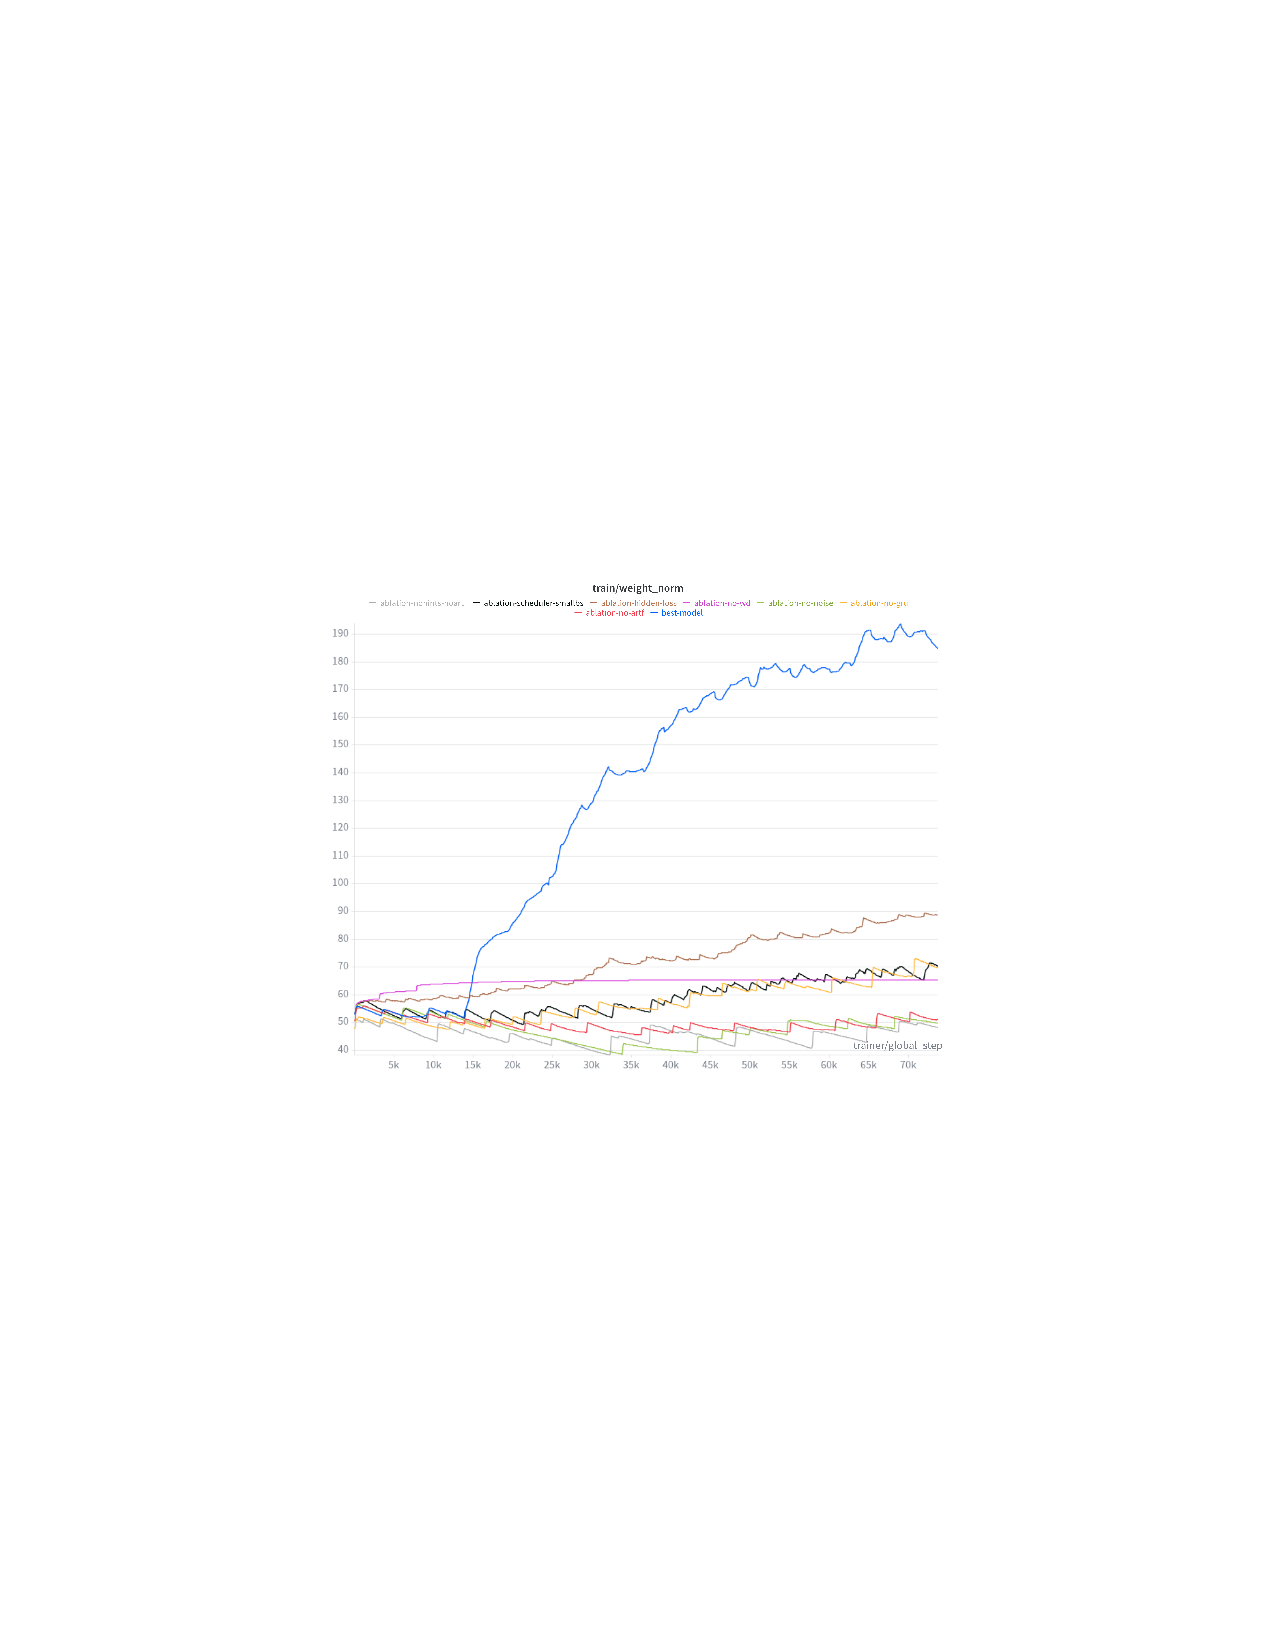
\includegraphics[trim={5.5cm 9.5cm 5.5cm 9.5cm}, clip, width=0.8\textwidth]{weight-norm-ablation.pdf}
  \caption{Training weight norm ($||w||$) progression. The low-variance baseline (\texttt{best-model}) successfully escapes the penalty phase to build a high-capacity circuit, whereas the small batch size (\texttt{ablation-scheduler-smallbs}) gets trapped at a lower norm.}
  \label{fig:weight_norm}
\end{figure}

\subsection{The Illusion of Learning (No Hints / No AR+TF)}

Removing step-by-step hints and AR+TF scaffolding (falling back to end-to-end training) induces a deceptive failure mode. We observe that while the end-to-end ablation (\texttt{ablation-nohints-noartf}) can achieve high validation node accuracy on Delaunay topologies (Figure \ref{fig:node_acc}), the metric is highly unstable, wildly oscillating between $0.80$ and $1.0$ during training. 

\begin{figure}[htbp]
  \centering
  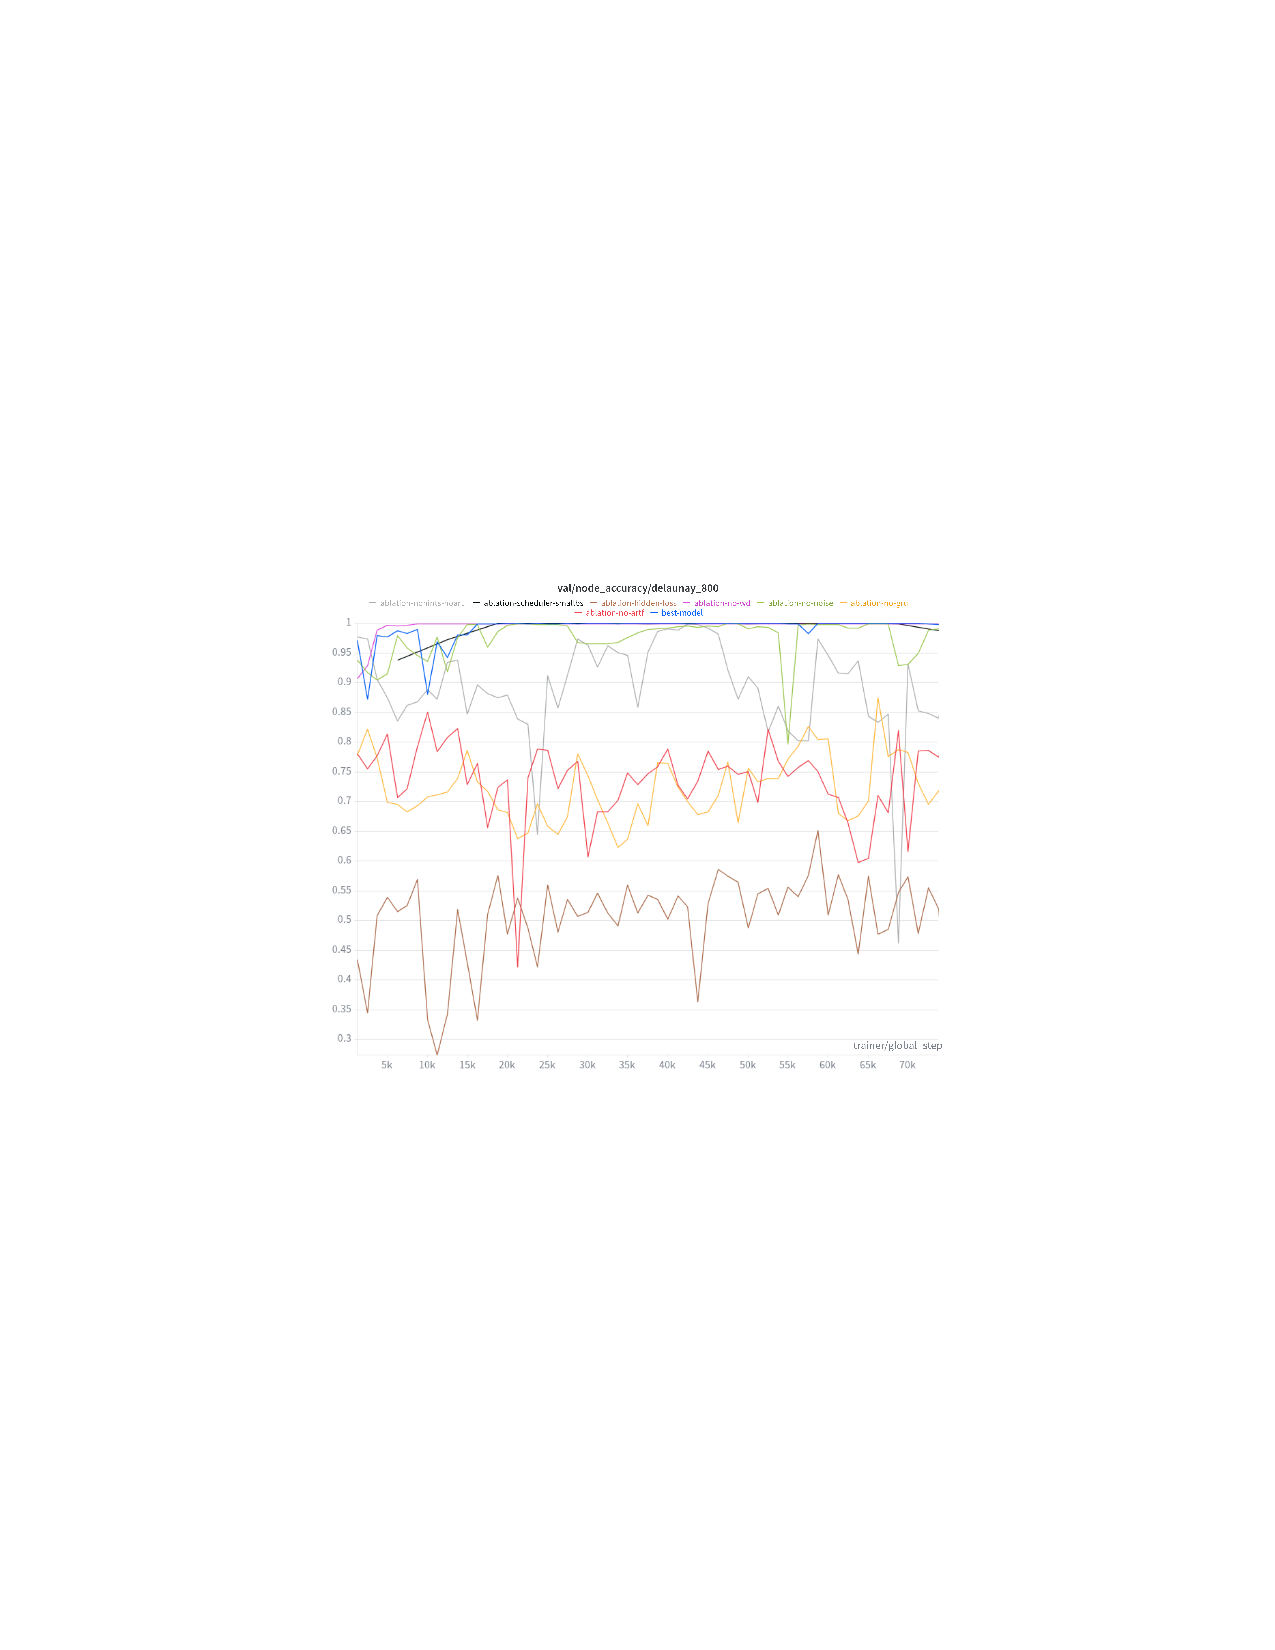
\includegraphics[trim={5.5cm 9.5cm 5.5cm 9.5cm}, clip, width=0.8\textwidth]{node_accuracy_de800-ablation.pdf}
  \caption{Validation Node Accuracy (Delaunay-800). The end-to-end ablation (\texttt{ablation-nohints-noartf}) exhibits thrashing compared to the stable \texttt{best-model}.}
  \label{fig:node_acc}
\end{figure}

Despite these localized spikes in node accuracy, the strict graph accuracy (Figure \ref{fig:graph_acc}) consistently flatlines at $0.0$. This discrepancy visually confirms that dense, step-by-step gradients from execution traces are empirically required to provide the structural scaffolding necessary for the model to align with the global algorithmic logic, rather than just overfitting to unstable local heuristics.

\begin{figure}[htbp]
  \centering
  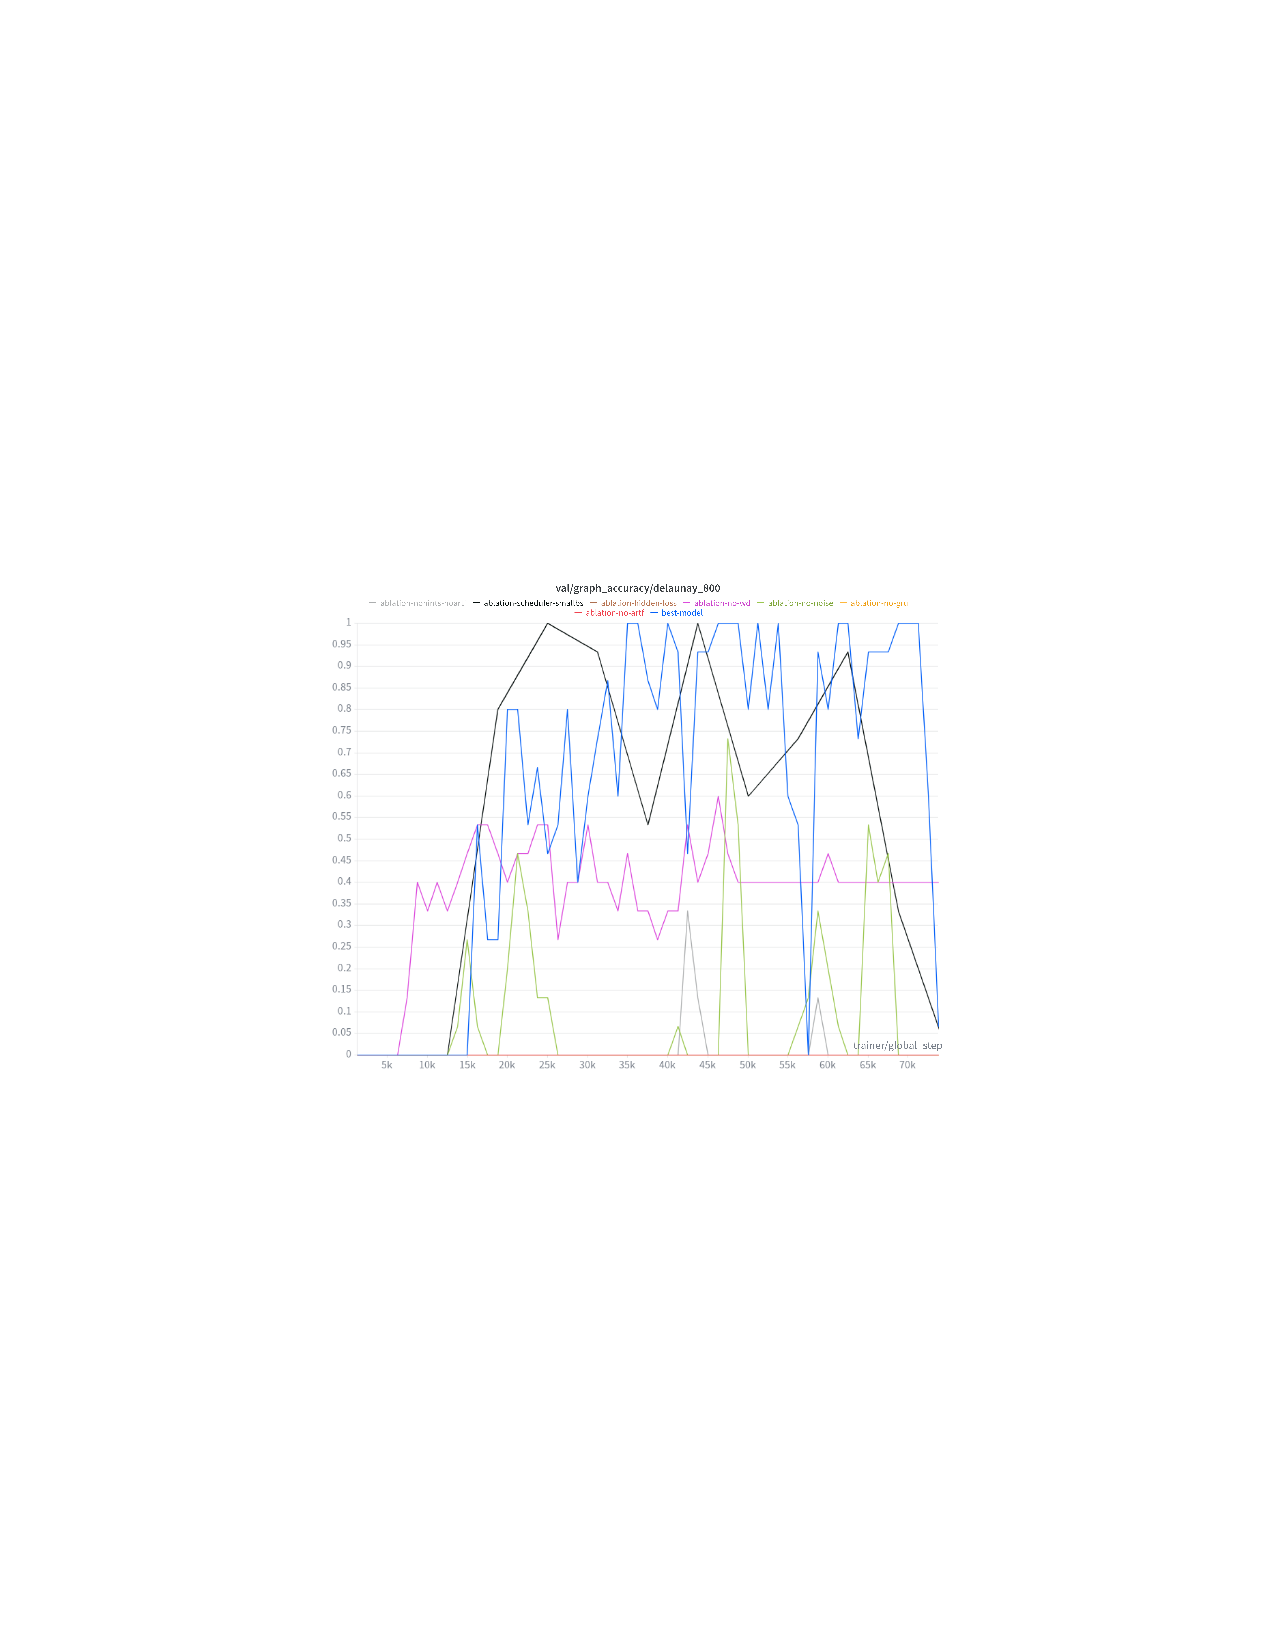
\includegraphics[trim={5.5cm 9.5cm 5.5cm 9.5cm}, clip, width=0.8\textwidth]{graph_accuracy_de800-ablation.pdf}
  \caption{Validation Graph Accuracy (Delaunay-800). Without step-by-step hints, the model completely fails to capture the strict structural logic of the BFS algorithm, flatlining at zero.}
  \label{fig:graph_acc}
\end{figure}

\subsection{Memory and Regularization Limitations}
\begin{itemize}
    \item \textbf{No GRU:} Fails catastrophically on Delaunay-800 graphs. Delaunay triangulations feature significantly larger graph diameters; without persistent GRU memory, the standard message-passing ``visited'' state likely dilutes and decays over long BFS depths.
    \item \textbf{No Weight Decay:} Removing the $L_2$ penalty traps the model in a stable local minimum of perfect training memorization, disabling the compression required for OOD graph accuracy.
    \item \textbf{No Hidden Noise:} The absence of hidden state noise degrades convergence speed and reduces strict graph accuracy on Watts-Strogatz topologies. Noise physically forces the model to learn to self-correct on long BFS trajectories, preventing microscopic errors from compounding over long rollouts.
    \item \textbf{Hidden Loss Trap:} Enforcing a direct $L_2$ loss on the hidden state creates a destructive information bottleneck, crippling the model's ability to store auxiliary spatial algorithmic memory (e.g., structural graph awareness), causing failure even on 80-node graphs.
\end{itemize}

\section{Per-Seed Results and Evaluation Precision}
\label{sec:perseed}

\paragraph{Evaluation precision.} The originally reported Table~1 was evaluated with fp16
autocast and reduced-precision (bf16) matrix multiplications, neither of which was stated.
Re-evaluating the same frozen best checkpoint on a fixed set of 200 graphs per bin, varying
only these two settings, strict graph accuracy is monotone in effective arithmetic
precision in every bin; the WS bins are by far the most sensitive:

\begin{table}[H]
  \caption{Strict graph accuracy of the best checkpoint under three effective evaluation
  precisions (same frozen weights, same 200 graphs per bin).}
  \label{precision-ladder}
  \centering
  \begin{tabular}{lcccccc}
    \toprule
    Effective precision & Del-800 & Del-1600 & ER-800 & ER-1600 & WS-800 & WS-1600 \\
    \midrule
    fp16 autocast (as originally reported) & 99.5 & 92.5 & 100.0 & 96.0 & 90.5 & 1.0 \\
    fp32, bf16 matmuls                     & 100.0 & 98.0 & 100.0 & 99.5 & 99.0 & 49.5 \\
    fp32, fp32 matmuls (used in Table~1)   & 100.0 & 100.0 & 100.0 & 99.5 & 99.5 & 98.0 \\
    \bottomrule
  \end{tabular}
\end{table}

\paragraph{Per-seed results.} Strict graph accuracy at full fp32 for all ten training runs
(200 graphs per bin). Grokked runs are identified by the training-time weight-norm
criterion of Section~3; the best checkpoint reported in Table~1 sits at the favourable end
of the grokked range and should not be read as typical.

\begin{table}[H]
  \caption{Per-seed strict graph accuracy (\%) at full fp32, 200 graphs per bin.}
  \label{per-seed-table}
  \centering
  \begin{tabular}{lccccccc}
    \toprule
    Seed & Grokked & Del-800 & Del-1600 & ER-800 & ER-1600 & WS-800 & WS-1600 \\
    \midrule
    42 & yes & 100.0 & 98.5 & 92.0 & 63.5 & 30.0 & 0.0 \\
    44 & yes & 100.0 & 99.5 & 100.0 & 100.0 & 81.5 & 2.5 \\
    46 & yes & 100.0 & 100.0 & 100.0 & 100.0 & 100.0 & 100.0 \\
    50 & yes & 100.0 & 100.0 & 100.0 & 100.0 & 100.0 & 57.0 \\
    51 & yes & 95.5 & 79.5 & 77.0 & 43.0 & 7.5 & 0.0 \\
    43 & no & 18.5 & 1.0 & 1.5 & 0.0 & 0.0 & 0.0 \\
    45 & no & 40.0 & 14.0 & 1.0 & 0.0 & 0.0 & 0.0 \\
    47 & no & 41.5 & 7.5 & 16.0 & 2.0 & 0.0 & 0.0 \\
    48 & no & 49.5 & 18.0 & 25.0 & 4.5 & 0.0 & 0.0 \\
    49 & no & 28.5 & 8.5 & 1.0 & 0.0 & 0.0 & 0.0 \\
    \midrule
    \multicolumn{2}{l}{mean $\pm$ std (grokked, $n{=}5$)} & $99.1 \pm 2.0$ & $95.5 \pm 9.0$ & $93.8 \pm 10.0$ & $81.3 \pm 26.6$ & $63.8 \pm 42.6$ & $31.9 \pm 45.2$ \\
    \bottomrule
  \end{tabular}
\end{table}

Performance remains topology-dependent at full precision (Delaunay $>$ ER $>$ WS at
$N{=}1600$), and variance across grokked seeds is large on the harder bins; both facts
temper, but do not overturn, the headline Delaunay result.

\section{Path-Graph Evaluation: Long Rollouts}
\label{sec:pathgraphs}

Path graphs are a demanding test of whether the model executes BFS rather than a
topology-exploiting heuristic: degree 2, zero clustering, no shortcuts, no planar or
geometric regularity, and rollouts far longer than any evaluation above (the rollout
length is $\max(s, n{-}1{-}s)$ for a uniformly random source $s$). Evaluated on the same
frozen best checkpoint at full fp32:

\begin{table}[H]
  \caption{Strict graph accuracy on path graphs at full fp32.}
  \label{path-table}
  \centering
  \begin{tabular}{lccc}
    \toprule
    Configuration & Strict graph acc. & Node acc. & Mean rollout steps \\
    \midrule
    path ($n{=}513$)  & 15/15 (100\%) & 100.0 & 375 \\
    path ($n{=}801$)  & 15/15 (100\%) & 100.0 & 606 \\
    path ($n{=}1201$) & 5/5 (100\%)   & 100.0 & 800 (max $\sim$1150) \\
    \bottomrule
  \end{tabular}
\end{table}

Under the originally used fp16 evaluation, the same configuration scores $0\%$ strict
accuracy at $n{=}801$: the model executes BFS exactly for hundreds of sequential steps on
a topology with no structural shortcut---each pointer depends on information up to
hundreds of hops away---and the earlier failure was arithmetic rather than algorithmic.

\end{document}